\documentclass{article}

% if you need to pass options to natbib, use, e.g.:
%     \PassOptionsToPackage{numbers, compress}{natbib}
% before loading neurips_2020

% ready for submission
% \usepackage{neurips_2020}

% to compile a preprint version, e.g., for submission to arXiv, add add the
% [preprint] option:
%     \usepackage[preprint]{neurips_2020}

% to compile a camera-ready version, add the [final] option, e.g.:
%     \usepackage[final]{neurips_2020}

% to avoid loading the natbib package, add option nonatbib:
\usepackage[nonatbib]{neurips_2020}

\usepackage[utf8]{inputenc} % allow utf-8 input
\usepackage[T1]{fontenc}    % use 8-bit T1 fonts
\usepackage{hyperref}       % hyperlinks
\usepackage{url}            % simple URL typesetting
\usepackage{booktabs}       % professional-quality tables
\usepackage{amsfonts}       % blackboard math symbols
\usepackage{nicefrac}       % compact symbols for 1/2, etc.
\usepackage{microtype}      % microtypography


%%%%我的包
\usepackage{graphicx}
%\graphicspath{ {./images/} }
\usepackage{float} 
\title{Report of face-recognition by finetuning ResNet}
\documentclass{article}
\usepackage[utf8]{inputenc}
\usepackage{booktabs} %三线表需要加载宏包{booktabs}
\usepackage{diagbox}
\usepackage{multirow}
\usepackage{listings}
\usepackage{xcolor}

%New colors defined below
\definecolor{codegreen}{rgb}{0,0.6,0}
\definecolor{codegray}{rgb}{0.5,0.5,0.5}
\definecolor{codepurple}{rgb}{0.58,0,0.82}
\definecolor{backcolour}{rgb}{0.95,0.95,0.92}

%Code listing style named "mystyle"
\lstdefinestyle{mystyle}{
  backgroundcolor=\color{backcolour},   commentstyle=\color{codegreen},
  keywordstyle=\color{magenta},
  numberstyle=\tiny\color{codegray},
  stringstyle=\color{codepurple},
  basicstyle=\ttfamily\footnotesize,
  breakatwhitespace=false,         
  breaklines=true,                 
  captionpos=b,                    
  keepspaces=true,                 
  numbers=left,                    
  numbersep=5pt,                  
  showspaces=false,                
  showstringspaces=false,
  showtabs=false,                  
  tabsize=2
}

%"mystyle" code listing set
\lstset{style=mystyle}



% The \author macro works with any number of authors. There are two commands
% used to separate the names and addresses of multiple authors: \And and \AND.
%
% Using \And between authors leaves it to LaTeX to determine where to break the
% lines. Using \AND forces a line break at that point. So, if LaTeX puts 3 of 4
% authors names on the first line, and the last on the second line, try using
% \AND instead of \And before the third author name.

\author{
   Haorui Li\thanks \\
  Chien-Shiung Wu College\\
  Southeast University\\
  % examples of more authors
  % \And
  % Coauthor \\
  % Affiliation \\
  % Address \\
  % \texttt{email} \\
  % \AND
  % Coauthor \\
  % Affiliation \\
  % Address \\
  % \texttt{email} \\
  % \And
  % Coauthor \\
  % Affiliation \\
  % Address \\
  % \texttt{email} \\
  % \And
  % Coauthor \\
  % Affiliation \\
  % Address \\
  % \texttt{email} \\
}

\begin{document}

\maketitle

\begin{abstract}
For face recognition, first, I use MTCNN and face.evoLVe for automatic data cleansing, then rename the folders by batch processing in order to fit the requirenments of Dataset.ImageFolder. Third, I trained two modles for face recognition, one is self-modified Resnet, another is InceptionResNetV1 with pre-trained weight, and finetuning the modle on classmates' data. Finally the best cross-entropy loss is 0.1830 and recognize 82/104 classmates.  
\end{abstract}

\section{Data prepare}
\subsection{Face alignment}
To begin with, I use MTCNN[1] and \textit{face.evoLVe.PyTorch} for automatic face alignment.

MTCNN propose a deep cascaded multi-task framework which
exploits the inherent correlation between them to boost up Resnet's performance on face alignment, the architecture is as follows:
\begin{figure}[H]%H为当前位置,!htb为忽略美学标准,htbp为浮动图形
  \centering
  \caption{MTCNN's architecture}
%可选参数中width=\columnwidth选取了当前列宽
  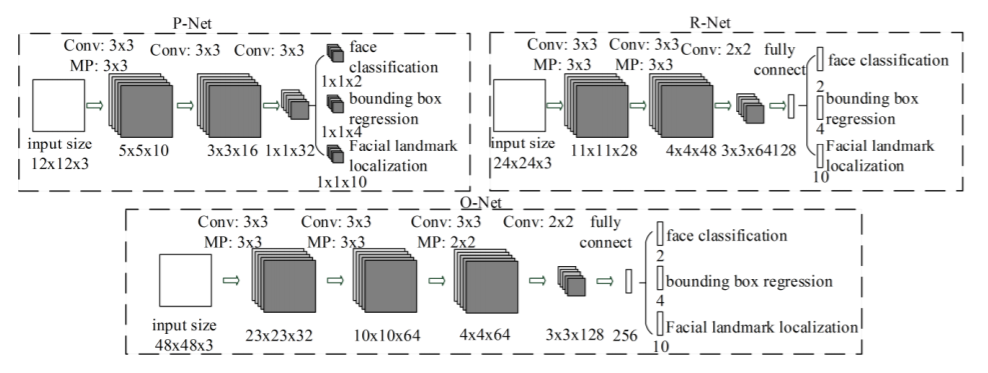
\includegraphics[width=\columnwidth]{IMG/MTCNN.png} %插入图片,[]中设置图片大小,{}中是图片文件名
  \label{Fig.RNN} %用于文内引用的标签
\end{figure}
Though MTCNN is very fast, but it sometimes go wrong and bring in dirty data, like the Figure2, and these dirty data will definitely bring catastrophe for model trainning.
\begin{figure}[H]%H为当前位置,!htb为忽略美学标准,htbp为浮动图形
  \centering
  \caption{Samples of dirty data by MTCNN}
%可选参数中width=\columnwidth选取了当前列宽
  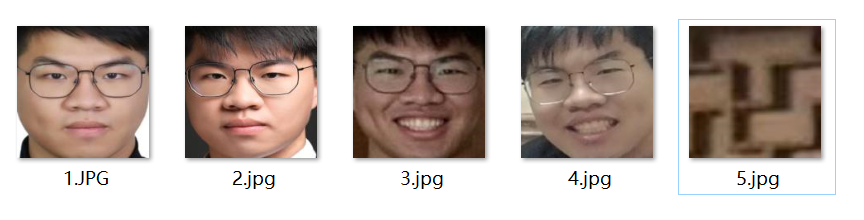
\includegraphics[width=\columnwidth]{IMG/ML大作业筛选展示.png} %插入图片,[]中设置图片大小,{}中是图片文件名
  \label{Fig.RNN} %用于文内引用的标签
\end{figure}
So I refer to \textit{face.evoLVe's face-align tools} and finally get good data.
This tool can be find at:
\begin{center}
  \url{https://github.com/ZhaoJ9014/face.evoLVe.PyTorch}
\end{center}
This tool is about 4-times slower than MTCNN, but brings no dirty data.
\subsection{Rebuild folder architecture}
For quick detect image labels, I use \textit{torchvision.datasets.ImageFolder} to automatically read classmates name. To use this function, I rebuild the data folder's architecture by code.

Exactly, I use os.rename and string.split. Following are some codes I use to split the student number:

\begin{lstlisting}[language=Python, caption=Change folder names for ImageFloder function]
def replaceDirName(rootDir):
  #Change the folders' name under rootDir, split the student number by '-' or '_'
    num = 0
    dirs = os.listdir(rootDir)
    for dir in dirs:
        print('oldname is:' + dir)
        num = num +1
        try:
          temp = dir.split('_')[1]
        except IndexError:
          try:
            temp=dir.split('-')[1]
          except:
            print("This is not Number-Name structure", dir)
            continue
        except:
          print("This is not - or _ structure", dir)
          continue
        print('new name:',temp)
        oldname = os.path.join(rootDir, dir)
        newname = os.path.join(rootDir, temp)
        os.rename(oldname, newname)#replace
replaceDirName('align_data')
\end{lstlisting}




After rebuild the folder architecture, \textit{torchvision.datasets.ImageFolder} is able to automatically read sub-folders' name as image label. 

\subsection{Transforms}
After clean the data and align all the faces, I made some extra preparations for models robustness and these work has brought about 3-point increase in test accuracy.

When load in the data I perform some random transforms to the images to improve training. Different transforms can be attempted and I tried various ones, like Random-Color-Jitter and Random-Rotation, along with Random-Horizontal-Flip.
\begin{figure}[H]%H为当前位置,!htb为忽略美学标准,htbp为浮动图形
  \centering
  \caption{Examples of random Color Jitter}
%可选参数中width=\columnwidth选取了当前列宽
  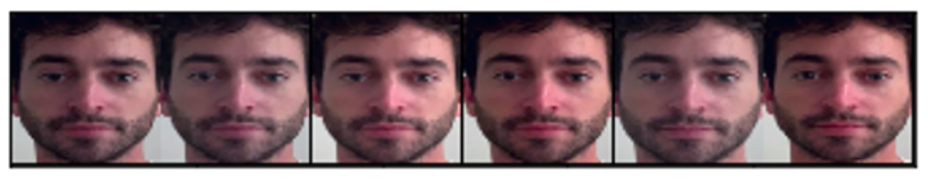
\includegraphics[width=\columnwidth]{IMG/随机彩色.png} %插入图片,[]中设置图片大小,{}中是图片文件名
  \label{Fig.RNN} %用于文内引用的标签
\end{figure}
Finally I choose all these transforms to improve the model's robustness. And the random-color-jitter improves about 2 points in accuracy probably because classmates take photo at different light environment.

\section{Design model architecture}
Due to the fact that the data we have is small scale, it will be hard to train a model without over-fitting. So I think it is recognized to use some pre-trained model and do the fine-tuning.  What I have to do is design the final layers.

\subsection{Pre-trained ResNet}
The pre-trained weight I download is the Facenet trained by Google. They use triple loss and finally get 0.997 accuracy at Lwf, the High-Level modal structure of Facenet is as follow[2]:
\begin{figure}[H]%H为当前位置,!htb为忽略美学标准,htbp为浮动图形
  \centering
  \caption{High Level Modal Structure of Facenet}
%可选参数中width=\columnwidth选取了当前列宽
  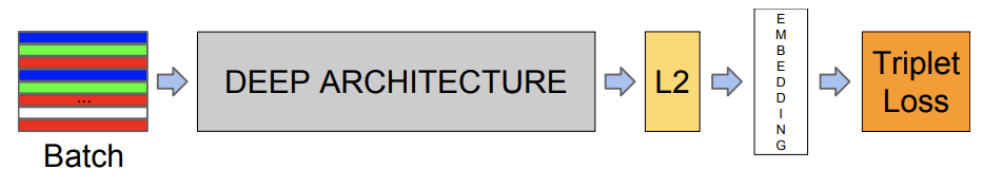
\includegraphics[width=\columnwidth]{IMG/facenet.png} %插入图片,[]中设置图片大小,{}中是图片文件名
  \label{Fig.RNN} %用于文内引用的标签
\end{figure}
And for the first model, I use Inception-ResNet[3] to fine-tuning the model, which is designed for fine-tuning Facenet. The architecture of Inception-ResNet is as follow:
\begin{figure}[H]%H为当前位置,!htb为忽略美学标准,htbp为浮动图形
  \centering
  \caption{Inception-ResNet}
%可选参数中width=\columnwidth选取了当前列宽
  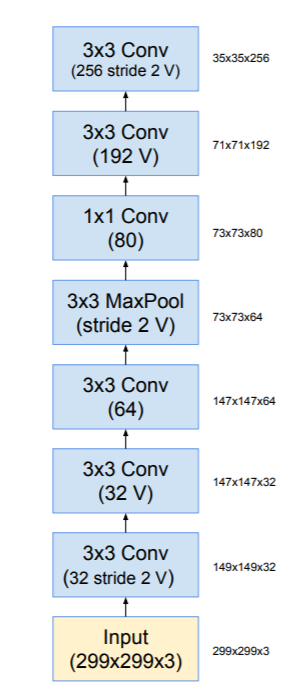
\includegraphics[width=18ex]{IMG/RESNET.png} %插入图片,[]中设置图片大小,{}中是图片文件名
  \label{Fig.RNN} %用于文内引用的标签
\end{figure}
The code of final layers are:
\begin{lstlisting}[language=Python, caption=Final layer Codes]
        self.block8 = Block8(noReLU=True)
        self.avgpool_1a = nn.AdaptiveAvgPool2d(1)
        self.dropout = nn.Dropout(dropout_prob)
        self.last_linear = nn.Linear(1792, 512, bias=False)
        self.last_bn = nn.BatchNorm1d(512, eps=0.001, momentum=0.1, affine=True)
        self.logits = nn.Linear(512, tmp_classes)
\end{lstlisting}
And I have modified the final layers to test which model is best.

\subsection{Modified ResNet}
From the upper section we can see the final six layers are:
\begin{lstlisting}[language=Python, caption=Final layers]
[Block8(
   (branch0): BasicConv2d(
     (conv): Conv2d(1792, 192, kernel_size=(1, 1), stride=(1, 1), bias=False)
     (bn): BatchNorm2d(192, eps=0.001, momentum=0.1, affine=True, track_running_stats=True)
     (relu): ReLU()
   )
   (branch1): Sequential(
     (0): BasicConv2d(
       (conv): Conv2d(1792, 192, kernel_size=(1, 1), stride=(1, 1), bias=False)
       (bn): BatchNorm2d(192, eps=0.001, momentum=0.1, affine=True, track_running_stats=True)
       (relu): ReLU()
     )
     (1): BasicConv2d(
       (conv): Conv2d(192, 192, kernel_size=(1, 3), stride=(1, 1), padding=(0, 1), bias=False)
       (bn): BatchNorm2d(192, eps=0.001, momentum=0.1, affine=True, track_running_stats=True)
       (relu): ReLU()
     )
     (2): BasicConv2d(
       (conv): Conv2d(192, 192, kernel_size=(3, 1), stride=(1, 1), padding=(1, 0), bias=False)
       (bn): BatchNorm2d(192, eps=0.001, momentum=0.1, affine=True, track_running_stats=True)
       (relu): ReLU()
     )
   )
   (conv2d): Conv2d(384, 1792, kernel_size=(1, 1), stride=(1, 1))
 ),
 AdaptiveAvgPool2d(output_size=1),
 Linear(in_features=1792, out_features=512, bias=False),
 BatchNorm1d(512, eps=0.001, momentum=0.1, affine=True, track_running_stats=True),
 Linear(in_features=512, out_features=8631, bias=True),
 Softmax(dim=1)]
\end{lstlisting}
Because earlier layers as containing the base-level information needed to recognize face attributes and base level characteristics, so I want to cut the layers after Conv2d and use some my own code, and just updating the final layers to include another 104 faces.

Put all beginning layers in an nn.Sequential:
\begin{lstlisting}[language=Python, caption=Keep the conv2d layers]
model_ft = nn.Sequential(*list(model_ft.children())[:-5])
\end{lstlisting}
Now, model modified is a torch model but without the final linear, pooling, batchnorm, and sigmoid layers.

After this, I design another final layers calss includs Flatten and Normalize, the codes are:
\begin{lstlisting}[language=Python, caption=Haorui Net]
#Change the final layers as follows
model_modified.avgpool_1a = nn.AdaptiveAvgPool2d(output_size=1)
model_modified.last_linear = nn.Sequential(
    Flatten(),
    nn.Linear(in_features=1792, out_features=512, bias=False),
    normalize()
)
model_modified.logits = nn.Linear(layer_list[4].in_features,104)
model_modified.softmax = nn.Softmax(dim=1)
model_modified = model_modified.to(device)
\end{lstlisting}
So the architecture is:
\begin{figure}[H]%H为当前位置,!htb为忽略美学标准,htbp为浮动图形
  \centering
  \caption{Haorui-Net Architecture}
%可选参数中width=\columnwidth选取了当前列宽
  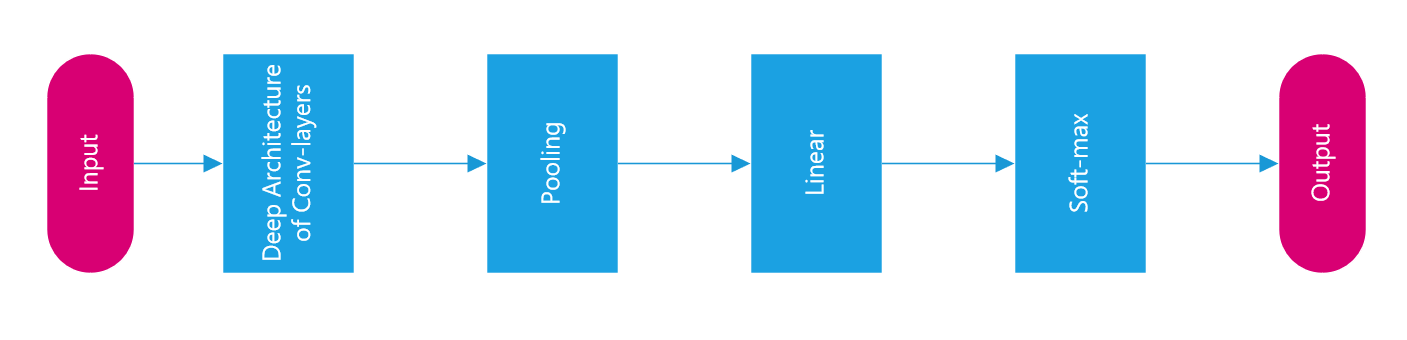
\includegraphics[width=\columnwidth]{IMG/haoruinet.png} %插入图片,[]中设置图片大小,{}中是图片文件名
  \label{Fig.RNN} %用于文内引用的标签
\end{figure}

We can name it Haorui-ResNet. In the next section I will train these two models and show some details to pick the winner.

\section{Training and preferences}
After design the model, I begin the training step. Tried different epoch, batch size, learning rate and models.
\subsection{Batch size and epochs}
The options of batch size are often limited by GPU memory.

On my machine, I have a  single Tesla-P-100 with 16280 MiB memory, which means I have more choice on batch size and epochs. 
\begin{figure}[H]%H为当前位置,!htb为忽略美学标准,htbp为浮动图形
  \centering
  \caption{24 Epochs and 64 Batch-size}
%可选参数中width=\columnwidth选取了当前列宽
  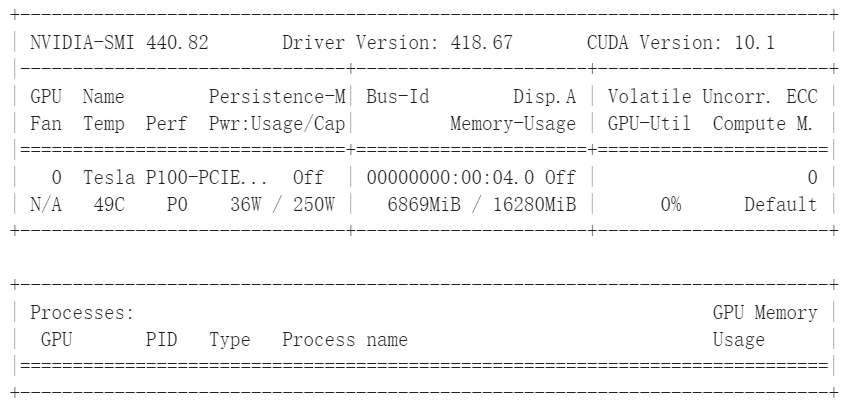
\includegraphics[width=\columnwidth]{IMG/ML实验GPU.png} %插入图片,[]中设置图片大小,{}中是图片文件名
  \label{Fig.RNN} %用于文内引用的标签
\end{figure}
After choose several combinations of epochs and batch size,  I get the results as follows on Inception-ResNet:

\begin{table}[!htbp]
\centering
\caption{Records of combination for ResNet}\label{tab:aStrangeTable}%添加标题 设置标签
\begin{tabular}{cccc}
\toprule
Epochs & Batch size& TP &Train FPS\\
\midrule
10& 16 & 21 & 427.4\\
24& 16& 26 & 420.7\\
24 & 32 & 41 & 279.6\\
24 & 64 & 75 & 153.4\\
32 & 64 & 71 & 161.5\\
24 & 128 & 80 & 149.5\\
32 & 128 & 77 & 233.9\\
24 & 256 & 70  &183.3\\
32 & 256 & 77  &192.8\\
64 & 256 & 76  &155.3\\
\bottomrule
\end{tabular}

%\caption{这是一张三线表}\label{tab:aStrangeTable}  标题放在这里也是可以的
\end{table}
From the chart we can see, more batch size often means better performance, but with more batch size, sometimes it need more epochs to minimize the loss, just like 256 batch size performs weaker than 128 batch size in 24 epochs, and become better in 32 epochs.

So finally, the ResNet performs its best at 24 epochs, 128 batch size and reaches 82 true positive. This model was saved as  '24-epoch-128bz-VGGFACE2-TEST80ACC.pb'.

With the chart above, I can qiuckly choose some combinations for Haorui-Net, and the results are as follows:

\begin{table}[!htbp]
\centering
\caption{Records of combination for Haorui-Net}\label{tab:aStrangeTable}%添加标题 设置标签
\begin{tabular}{cccc}
\toprule
Epochs & Batch size& TP &Train FPS\\
\midrule
24 & 128 & 82 & 171.4\\
32 & 128 & 76 & 255.5\\
\bottomrule
\end{tabular}
\end{table}

Luckily, the Haorui-Net performs better than ResNet its best at 24 epochs, 128 batch size and reaches 82 true positive. This model was saved as  '24-epoch-128bz-MODIFIED-TEST82ACC.pb'.

So I'm proud to announce that Haorui-Net becomes the winner in this combination, with two more ture-positive!

But what I want to point out is that, Haorui-Net is weaker in the decrease of loss, for ResNet, the minimum of loss is about 0.27 while training, but for Haorui-Net, the minimum loss is about 3.8, it probably means ResNet is designed more smarter in track and reduce the loss.


%%%%%%%%%%%%%%%%%%%%%%%%%%%%%%%%
The style files for NeurIPS and other conference information are available on
the World Wide Web at
\begin{center}
  \url{http://www.neurips.cc/}
\end{center}
The file \verb+neurips_2020.pdf+ contains these instructions and illustrates the
various formatting requirements your NeurIPS paper must satisfy.

The only supported style file for NeurIPS 2020 is \verb+neurips_2020.sty+,
rewritten for \LaTeXe{}.  \textbf{Previous style files for \LaTeX{} 2.09,
  Microsoft Word, and RTF are no longer supported!}

The \LaTeX{} style file contains three optional arguments: \verb+final+, which
creates a camera-ready copy, \verb+preprint+, which creates a preprint for
submission to, e.g., arXiv, and \verb+nonatbib+, which will not load the
\verb+natbib+ package for you in case of package clash.

\paragraph{Preprint option}
If you wish to post a preprint of your work online, e.g., on arXiv, using the
NeurIPS style, please use the \verb+preprint+ option. This will create a
nonanonymized version of your work with the text ``Preprint. Work in progress.''
in the footer. This version may be distributed as you see fit. Please \textbf{do
  not} use the \verb+final+ option, which should \textbf{only} be used for
papers accepted to NeurIPS.

At submission time, please omit the \verb+final+ and \verb+preprint+
options. This will anonymize your submission and add line numbers to aid
review. Please do \emph{not} refer to these line numbers in your paper as they
will be removed during generation of camera-ready copies.

The file \verb+neurips_2020.tex+ may be used as a ``shell'' for writing your
paper. All you have to do is replace the author, title, abstract, and text of
the paper with your own.

The formatting instructions contained in these style files are summarized in
Sections \ref{gen_inst}, \ref{headings}, and \ref{others} below.

\section{General formatting instructions}
\label{gen_inst}

The text must be confined within a rectangle 5.5~inches (33~picas) wide and
9~inches (54~picas) long. The left margin is 1.5~inch (9~picas).  Use 10~point
type with a vertical spacing (leading) of 11~points.  Times New Roman is the
preferred typeface throughout, and will be selected for you by default.
Paragraphs are separated by \nicefrac{1}{2}~line space (5.5 points), with no
indentation.

The paper title should be 17~point, initial caps/lower case, bold, centered
between two horizontal rules. The top rule should be 4~points thick and the
bottom rule should be 1~point thick. Allow \nicefrac{1}{4}~inch space above and
below the title to rules. All pages should start at 1~inch (6~picas) from the
top of the page.

For the final version, authors' names are set in boldface, and each name is
centered above the corresponding address. The lead author's name is to be listed
first (left-most), and the co-authors' names (if different address) are set to
follow. If there is only one co-author, list both author and co-author side by
side.

Please pay special attention to the instructions in Section \ref{others}
regarding figures, tables, acknowledgments, and references.

\section{Headings: first level}
\label{headings}

All headings should be lower case (except for first word and proper nouns),
flush left, and bold.

First-level headings should be in 12-point type.

\subsection{Headings: second level}

Second-level headings should be in 10-point type.

\subsubsection{Headings: third level}

Third-level headings should be in 10-point type.

\paragraph{Paragraphs}

There is also a \verb+\paragraph+ command available, which sets the heading in
bold, flush left, and inline with the text, with the heading followed by 1\,em
of space.

\section{Citations, figures, tables, references}
\label{others}

These instructions apply to everyone.

\subsection{Citations within the text}

The \verb+natbib+ package will be loaded for you by default.  Citations may be
author/year or numeric, as long as you maintain internal consistency.  As to the
format of the references themselves, any style is acceptable as long as it is
used consistently.

The documentation for \verb+natbib+ may be found at
\begin{center}
  \url{http://mirrors.ctan.org/macros/latex/contrib/natbib/natnotes.pdf}
\end{center}
Of note is the command \verb+\citet+, which produces citations appropriate for
use in inline text.  For example,
\begin{verbatim}
   \citet{hasselmo} investigated\dots
\end{verbatim}
produces
\begin{quote}
  Hasselmo, et al.\ (1995) investigated\dots
\end{quote}

If you wish to load the \verb+natbib+ package with options, you may add the
following before loading the \verb+neurips_2020+ package:
\begin{verbatim}
   \PassOptionsToPackage{options}{natbib}
\end{verbatim}

If \verb+natbib+ clashes with another package you load, you can add the optional
argument \verb+nonatbib+ when loading the style file:
\begin{verbatim}
   \usepackage[nonatbib]{neurips_2020}
\end{verbatim}

As submission is double blind, refer to your own published work in the third
person. That is, use ``In the previous work of Jones et al.\ [4],'' not ``In our
previous work [4].'' If you cite your other papers that are not widely available
(e.g., a journal paper under review), use anonymous author names in the
citation, e.g., an author of the form ``A.\ Anonymous.''

\subsection{Footnotes}

Footnotes should be used sparingly.  If you do require a footnote, indicate
footnotes with a number\footnote{Sample of the first footnote.} in the
text. Place the footnotes at the bottom of the page on which they appear.
Precede the footnote with a horizontal rule of 2~inches (12~picas).

Note that footnotes are properly typeset \emph{after} punctuation
marks.\footnote{As in this example.}

\subsection{Figures}



All artwork must be neat, clean, and legible. Lines should be dark enough for
purposes of reproduction. The figure number and caption always appear after the
figure. Place one line space before the figure caption and one line space after
the figure. The figure caption should be lower case (except for first word and
proper nouns); figures are numbered consecutively.

You may use color figures.  However, it is best for the figure captions and the
paper body to be legible if the paper is printed in either black/white or in
color.

\subsection{Tables}

All tables must be centered, neat, clean and legible.  The table number and
title always appear before the table.  See Table~\ref{sample-table}.

Place one line space before the table title, one line space after the
table title, and one line space after the table. The table title must
be lower case (except for first word and proper nouns); tables are
numbered consecutively.

Note that publication-quality tables \emph{do not contain vertical rules.} We
strongly suggest the use of the \verb+booktabs+ package, which allows for
typesetting high-quality, professional tables:
\begin{center}
  \url{https://www.ctan.org/pkg/booktabs}
\end{center}
This package was used to typeset Table~\ref{sample-table}.

\begin{table}
  \caption{Sample table title}
  \label{sample-table}
  \centering
  \begin{tabular}{lll}
    \toprule
    \multicolumn{2}{c}{Part}                   \\
    \cmidrule(r){1-2}
    Name     & Description     & Size ($\mu$m) \\
    \midrule
    Dendrite & Input terminal  & $\sim$100     \\
    Axon     & Output terminal & $\sim$10      \\
    Soma     & Cell body       & up to $10^6$  \\
    \bottomrule
  \end{tabular}
\end{table}

\section{Final instructions}

Do not change any aspects of the formatting parameters in the style files.  In
particular, do not modify the width or length of the rectangle the text should
fit into, and do not change font sizes (except perhaps in the
\textbf{References} section; see below). Please note that pages should be
numbered.

\section{Preparing PDF files}

Please prepare submission files with paper size ``US Letter,'' and not, for
example, ``A4.''

Fonts were the main cause of problems in the past years. Your PDF file must only
contain Type 1 or Embedded TrueType fonts. Here are a few instructions to
achieve this.

\begin{itemize}

\item You should directly generate PDF files using \verb+pdflatex+.

\item You can check which fonts a PDF files uses.  In Acrobat Reader, select the
  menu Files$>$Document Properties$>$Fonts and select Show All Fonts. You can
  also use the program \verb+pdffonts+ which comes with \verb+xpdf+ and is
  available out-of-the-box on most Linux machines.

\item The IEEE has recommendations for generating PDF files whose fonts are also
  acceptable for NeurIPS. Please see
  \url{http://www.emfield.org/icuwb2010/downloads/IEEE-PDF-SpecV32.pdf}

\item \verb+xfig+ "patterned" shapes are implemented with bitmap fonts.  Use
  "solid" shapes instead.

\item The \verb+\bbold+ package almost always uses bitmap fonts.  You should use
  the equivalent AMS Fonts:
\begin{verbatim}
   \usepackage{amsfonts}
\end{verbatim}
followed by, e.g., \verb+\mathbb{R}+, \verb+\mathbb{N}+, or \verb+\mathbb{C}+
for $\mathbb{R}$, $\mathbb{N}$ or $\mathbb{C}$.  You can also use the following
workaround for reals, natural and complex:
\begin{verbatim}
   \newcommand{\RR}{I\!\!R} %real numbers
   \newcommand{\Nat}{I\!\!N} %natural numbers
   \newcommand{\CC}{I\!\!\!\!C} %complex numbers
\end{verbatim}
Note that \verb+amsfonts+ is automatically loaded by the \verb+amssymb+ package.

\end{itemize}

If your file contains type 3 fonts or non embedded TrueType fonts, we will ask
you to fix it.

\subsection{Margins in \LaTeX{}}

Most of the margin problems come from figures positioned by hand using
\verb+\special+ or other commands. We suggest using the command
\verb+\includegraphics+ from the \verb+graphicx+ package. Always specify the
figure width as a multiple of the line width as in the example below:
\begin{verbatim}
   \usepackage[pdftex]{graphicx} ...
   \includegraphics[width=0.8\linewidth]{myfile.pdf}
\end{verbatim}
See Section 4.4 in the graphics bundle documentation
(\url{http://mirrors.ctan.org/macros/latex/required/graphics/grfguide.pdf})

A number of width problems arise when \LaTeX{} cannot properly hyphenate a
line. Please give LaTeX hyphenation hints using the \verb+\-+ command when
necessary.


\section*{Broader Impact}

Authors are required to include a statement of the broader impact of their work, including its ethical aspects and future societal consequences. 
Authors should discuss both positive and negative outcomes, if any. For instance, authors should discuss a) 
who may benefit from this research, b) who may be put at disadvantage from this research, c) what are the consequences of failure of the system, and d) whether the task/method leverages
biases in the data. If authors believe this is not applicable to them, authors can simply state this.

Use unnumbered first level headings for this section, which should go at the end of the paper. {\bf Note that this section does not count towards the eight pages of content that are allowed.}

\begin{ack}
Use unnumbered first level headings for the acknowledgments. All acknowledgments
go at the end of the paper before the list of references. Moreover, you are required to declare 
funding (financial activities supporting the submitted work) and competing interests (related financial activities outside the submitted work). 
More information about this disclosure can be found at: \url{https://neurips.cc/Conferences/2020/PaperInformation/FundingDisclosure}.


Do {\bf not} include this section in the anonymized submission, only in the final paper. You can use the \texttt{ack} environment provided in the style file to autmoatically hide this section in the anonymized submission.
\end{ack}

\section*{References}

References follow the acknowledgments. Use unnumbered first-level heading for
the references. Any choice of citation style is acceptable as long as you are
consistent. It is permissible to reduce the font size to \verb+small+ (9 point)
when listing the references.
{\bf Note that the Reference section does not count towards the eight pages of content that are allowed.}
\medskip

\small

[1] Zhang, K., Zhang, Z., Li, Z. & Qiao, Y. (2016). Joint Face Detection and Alignment using Multi-task Cascaded Convolutional Networks.. CoRR, abs/1604.02878.
[2]Schroff, F., Kalenichenko, D. & Philbin, J. (2015). FaceNet: A Unified Embedding for Face Recognition and Clustering (cite arxiv:1503.03832Comment: Also published, in Proceedings of the IEEE Computer Society Conference on Computer Vision and Pattern Recognition 2015)
[3]Szegedy, C., Ioffe, S., Vanhoucke, V. & Alemi, A. A. (2017). Inception-v4, Inception-ResNet and the Impact of Residual Connections on Learning. Proceedings of the 31st AAAI Conference on Artificial Intelligence (p./pp. 4278--4284), : AAAI Press.




\end{document}
